\chapter{LDoS攻击原理与形式介绍}
\label{cha:LDoS}

本章的主要内容是对LDoS攻击进行探讨。首先对LDoS攻击原理进行说明。接下来,对LDoS攻击模型进行分析与说明。最后,对LDoS攻击的各类攻击形式进行分析和探讨。

\section{LDoS攻击原理}
\label{chap3:LDoSstate}

\subsection{TCP拥塞控制机制和超时重传机制}

此部分的主要内容为分析传输控制协议(Transmission Control Protocol,TCP)的拥塞控制机制与超时重传机制。首先讨论了不同时期提出的TCP拥塞控制机制,然后对超时重传机制(Retransmission Time Out, RTO)进行分析,探讨超时重传机制对TCP流的影响。

TCP协议是保证数据可靠的协议。对于任何基于TCP协议的数据流,都需要TCP拥塞控制机制,因为该机制可以对网络进行有效的调节。在网络中,所有的流都想让自己的数据尽快的传输,但是,所有流尽可能传输的结果就可能造成路由器或者链路的负载过大,引发网络拥塞,所有流都无法传输数据。因此,网络拥塞控制对于网络是必不可少的,而TCP拥塞控制为了给TCP流争提供合适的竞争方式。

TCP拥塞控制在TCP协议中实现,在传输层实现。TCP拥塞控制机制也并非一成不变的,针对不同的场景,TCP拥塞控制的策略也会不同,很多研究对TCP拥塞控制机制进行了探索。

最早的拥塞控制机制是1988年由Jacobson.V\cite{Jacobson1988Congestion}提出的TCP Reno版本,该方案的主要是由慢启动、拥塞避免、快重传和快恢复四个部分组成,大部分的拥塞控制方案都是以该方案作为基础进行提升的,由于该方案设计的时候有些方面未曾考虑,因此,该方案适用于低延迟、低带宽的网络。
在1994年由O’Malley.S.W\cite{O1994TCP}提出的TCP Vegas版本,该方案通过RTT来精准的预测带宽的变化,判断网络的可用带宽。不过,该方案适用于只存在这一种算法的时候。
在2008年,由Ha.S\cite{Ha2008CUBIC}提出的TCP Cubic方案,该方案使用立方函数作为拥塞窗口的增长函数,因此能够在不出现丢包的情况下,保持自己的传输速率。该方案能够尽可能的利用网络剩余带宽,适用于高带宽、丢包少的网络。
2017年由Cardwell.N\cite{Cardwell2017BBR}提出的TCP BBR版本,该算法在谷歌使用之后,极大的提升了数据传输性能。该算法认为当网络中的数据包总量高于网络中可存放数据包总量的时候会产生拥塞,就会限制窗口,因此,在带宽高、延迟高还有一定丢包率的情况下,降低时延并且保证带宽。
此外,2013年由Winstein.K\cite{Winstein2013Remy}提出的Remy算法采用机器学习的方式生成拥塞控制形式。因此,该算法适用于挽留过复杂的网络环境。

拥塞控制机制并非一成不变的,不同的方案有不同的适应场景,但是,这些方案都遵循着超时重传机制。在网络极其拥塞的情况下,TCP协议的发送端与接收端都收不到数据包,此时为了保证数据稳定的传输,TCP协议的发送端会进入指数退避阶段,将发送窗口改为1,避免网络进一步拥塞。在超时重传机制中,TCP流依靠RTO计时器来不定期探测网络拥塞状况。在TCP协议运行的过程中,RTO计时器中的值是由根据RTT实时计算得到的。

TCP的发送端维持两个两个变量,平滑往返时间(Smoothed Round-Trip Time, SRTT)和往返时间变化量(Round-Trip Time VARiation, RTTVAR)。根据RFC2988\cite{2000Computing}的设定,RTO的实时计算结果与SRTT、RTTVAR两个变量相关。当TCP的发送端与接收端完成一次测量RTT之后,发送端将RTO计时器设置为3秒。
当第一次测量获得的RTT,$R'$,主机设置SRTT = $R'$,RTTVAR = $R' / 2$,RTO = SRTT + max(G, 4RTTVAR),此处的G被标记为时钟粒度(一般情况下,$\leq$100毫秒)。当获得一个RTT的值$R'$之后,RTTVAR和SRTT的计算公式如下:


\begin{center}
    RTTVAR = (1 - $\beta$) RTTVAR + $\beta$ |SRTT - $R'$|
\vspace{-0.1in}
\end{center}

\begin{center}
    SRTT = (1 - $\alpha$) SRTT + $\alpha R'$
\end{center}

其中,有文献\cite{Jacobson1988Congestion}推荐设置$\alpha$ = 1/8, $\beta$ = 1/4。


通过对RTTVAR和SRTT进行跟新之后,TCP发送端RTO的计算公式如下:
\begin{center}
    RTO = max(minRTO, SRTT + max(G,4 RTTVAR)).
\end{center}

在Linux系统中,一般讲RTO计时器的最小值(minRTO)设置为0.2秒,因此,在推荐的参数中,延迟低的网络RTO基本是0.2秒。

接下来,对超时重传管理机制通过RTO计时器进行控制的流程进行分析。若是在某一时刻$t_0$,一个序号为$n$的数据包有TCP的发送端发送,此时一个初始值设为0.2秒的RTO计时器开始计时,如果$n$号的数据包丢失了或者说接收端重复发送的三个ACK包都没被发送包接收。当RTO计时器算到0.2秒的时候,则这个流就会被认为超时。此时,发送端进入指数退避阶段,发送端将拥塞控制的窗口置为1,并且让RTO计时器的值加倍,变为400毫秒,重传序号为$n$的未曾接收到ACK的数据包,并且重置RTO计时器为新的RTO的值。

若是序号为$n$的数据包再次丢失,则发送端持续保持,发送端将保持在指数退避阶段,而RTO计时器将会等待400毫秒。也就是说在$t_0$ + 0.6s的时候,RTO的值将被设为800毫秒,并重复此过程。

若是序号为$n$的数据包的数据包成功的$t_0$ + 0.2s之前接收到该数据包,例如在$t$+ RTT的时刻接收到$n$号数据包,则TCP发送端退出指数退避阶段并将RTO的值置为0.2秒,又开始正常的传输。

\subsection{LDoS攻击原理}
此部分的主要内容为LDoS攻击原理进行分析,讲述如何利用TCP的超时重传机制对来实现DoS攻击。

上述的超时机制对于拥塞控制是十分重要的,因为在网络十分拥塞的情况下,发送少量的数据包先进行探测网络的可达性是必要的。但是,这样的超时重传机制也会给网络带来很大的风险,比如给特定的低速率攻击能够利用该机制对TCP流产生极大的影响。

若是一个攻击者针对TCP流,通过发送周期性的短时间高速突发来迫使该流重复进入超时重传状态。攻击的突发持续时间必须得超过RTT的时间,需要RTO为攻击的周期的整数倍数,例如,RTO,RTO/2,RTO/3等。受害者的吞吐量被限制待到近乎为0的程度。与此同时,由于该攻击的平均速率较低,不容易被DoS的对抗机制所检测。

\begin{figure}
    \centering
    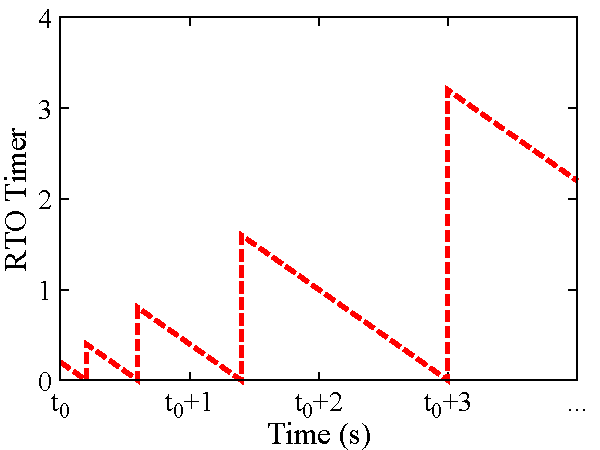
\includegraphics[scale=0.75]{RTO_timer}
    \caption{$t_0$时刻发动LDoS攻击之后,RTO计时器变化情况}
    \label{fig:rto-timer}
\end{figure}

首先考虑最简单的情况,若是一个攻击者仅仅针对一条TCP流进行攻击,攻击者在$t_0$时刻开始展开攻击,开始发送短时间的高速突发,就像\ref{fig:rto-timer}展示的那样,根据RTO计时器的初始值为0.2秒,该TCP流会等待0.2秒。如果攻击者在$t_0$ + 0.2和$t_0$ + 0.2 + 2RTT的时间内进行短时间的突发流进行攻击,则TCP流将不得不等待额外的0.4秒。通过在$t$= $t_0$ + 0.6, $t_0$ + 1.4等点创造类似的攻击,就能够不断迫使该TCP流进入超时重传状态。因此,可以得到针对某一特定TCP流的DoS攻击流的形式,如图\ref{fig:rate-min-LDoS}所示。

\begin{figure}
    \centering
    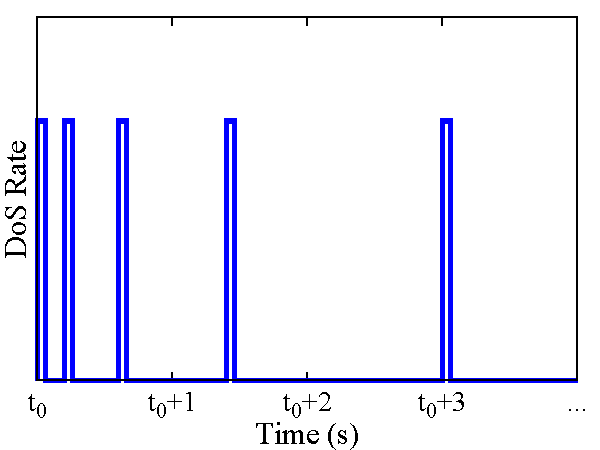
\includegraphics[scale=0.75]{rate-min-LDoS}
    \caption{高效的低速攻击方案}
    \label{fig:rate-min-LDoS}
\end{figure}

图\ref{fig:rate-min-LDoS}的攻击形式能够以最小的平均攻击速率使一个TCP流不断进入超时重传状态。但是,该形式却存在一个很大的弊端,若是在某一次攻击突发没有让ACK包被丢弃,则RTO计时器会重置为初始值,这样会使得该形式失效。因此,该形式虽然效率高,平均速率低,但是,并不适合于用作LDoS的基础形式。


\section{LDoS攻击模型}
\label{LDoS-model}
LDoS攻击形式需要一定的稳定性,不能因为偶尔出现的特殊情况就失去效果,考虑到这一点,使用周期性的的“方波”作为LDoS攻击的基础形式能够获得比较好的效果,如图\ref{fig:LDoS}所示。其中,攻击者可以通过发送周期为$T$,每次突发持续时间为$L$,速率为$R$的LDoS攻击流来对TCP流进行攻击。不过,想要LDoS攻击对TCP流有效果是需要满足一定的条件的。首先,速率$R$必须足够大来引起丢包,也就是说,$R$与其他的流量混合起来一定要超过链路容量。其次,突发持续时间$L$必须足够长来引起丢包,但是也要足够短来避免检测。还有周期$T$也要与RTO成比例关系,这样当TCP流想要退出超时重传状态的时候,就不得不丢包,从而保持超时重传状态。

\begin{figure}
    \centering
    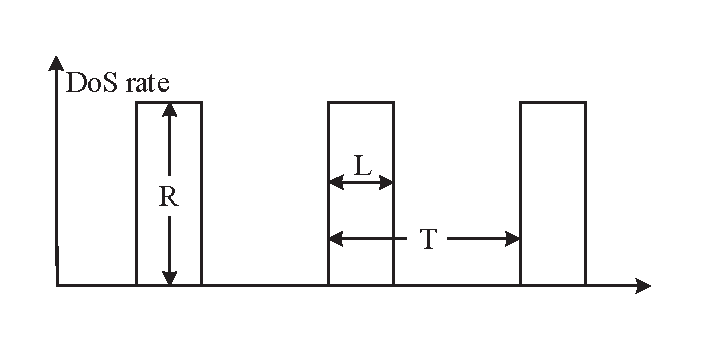
\includegraphics[scale=0.75]{LDoS}
    \caption{LDoS攻击形式}
    \label{fig:LDoS}
\end{figure}

前面讨论了针对一条攻击流的考虑LDoS攻击的情景,我们可以得到LDoS攻击模型,如图\ref{fig:model}所示,n条拥有不同RTT的TCP流和一条LDoS攻击流通过一个瓶颈队列。将RTT$_{i}$标记为第i条TCP流的RTT,其中i=1,…,$n$。LDoS攻击起效需要满足下面的条件:
\begin{itemize}
    \item 突发持续时间$L \geq RTT_i $
    \item minRTO > SRTT$_i$ + 4*RTTVAR$_i$
\end{itemize}

通过之前的分析可以得出一个结论,周期性的高速突发能够创造一段“停滞”状态,在这种状态下,丢包率很高,如果这种状态维持的时间超过RTT的时间规模,即$L \geq RTT_i$,对i=1,…,$n$,则由LDoS的攻击突发引起的拥塞将维持足够长的时间来迫使所有的TCP流进入超时重传状态。除此之外,当且仅当minRTO > SRTT$_i$ + 4*RTTVAR$_i$的时候,则所有TCP流的RTO计时器的值就会统一为minRTO,这样攻击者就能够知道TCP流的RTO计时器的值。在这种情况下,我们能够排除影响LDoS攻击的两个重要的问题,第一个问题是不同的TCP流RTT不同;第二个问题是不同的TCP流RTO计时器的值不同的问题。这样,LDoS攻击就能够对满足这两个条件的TCP流进行攻击。

\begin{figure}
    \centering
    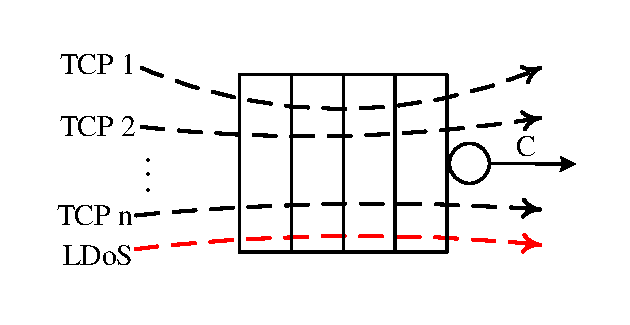
\includegraphics[scale=1]{queue}
    \caption{LDoS攻击模型}
    \label{fig:model}
\end{figure}

接下来,考虑如果有TCP流不满足上述两个条件其中任何一个甚至两个都不满足,LDoS攻击的效果就会不一样。如果一些TCP流只有一部分满足上面两个条件,则他们的吞吐量将会降低至近乎为0的程度,而不满足上述条件的则吞吐量下降,下降的之后的标准化吞吐量由公式\ref{equ:thputsurvive}来描述。

\begin{equation}
    \label{equ:thputsurvive}
    NT = \frac{\lceil \frac{minRTO}{T}\rceil T - minRTO}{T}.
\end{equation}

